\documentclass[hyperref, UTF8]{ctexart}

\usepackage{fullpage}
\usepackage{float}

\usepackage{xcolor}
\hypersetup{colorlinks=true, linkcolor=black, urlcolor=blue, unicode=true}

% For show image
\usepackage{graphicx}
\usepackage{caption}
\usepackage{subcaption}

\usepackage{tikz}
\usepackage{amsmath}

%-----------------Algorithm Packages--------------------
\usepackage{listings}                        % Source code
\usepackage{algorithm}                    % Pseudo Code
\usepackage{algpseudocode}
%---------------------------------------------------------

\title{数据挖掘课程项目 \\
	Large Scale Classification}
\author{
	数字媒体与技术, 13331043 \\
	戴旋  (\href{mailto:daixuan1996@gmail.com}{daixuan1996@gmail.com})}
\date{\today}

\begin{document}

\maketitle
\tableofcontents

\section{问题描述}

数据集中包含\ 2177020 条记录用作训练,以及\ 220245 条记录用作测试。每条记录中都包含\ 11392 个特征,每个特征的值为 0 与 1。以及一个分类参考值,为\ 0 或\ 1。任务目标是通过给定的数据集训练一个分类器来尽可能精准地为测试数据分类。

\section{实现方法}

考虑到每个记录只有两类,使用线性回归分类应是可行的。而参数调优简单地梯度下降即可完成。由于数据量庞大,特性很多,需要采取措施来减少处理的特性数量,可做一下映射。至于并行化,考虑到本机状况,可采用\ OpenMP 达成。

\subsection{线性回归分类}

首先我们采用的 sigmoid 函数为:$g(z) = \frac{1}{1 + e^{-z}}$。它的函数图像如下:

\begin{center}
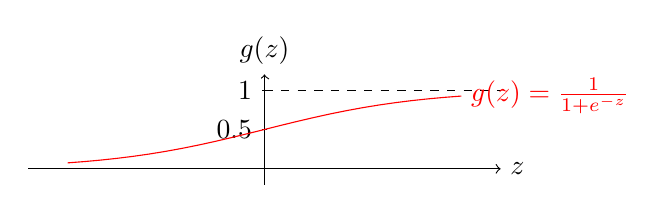
\begin{tikzpicture}
  \draw[->] (-3.0, 0) -- (3.0, 0) node[right] {$z$};
  \draw[->] (0, -0.2) -- (0, 1.2) node[above] {$g(z)$};
  \draw (1pt, 1cm) -- (-1pt, 1cm) node[anchor=east, fill=white] {$1$};
  \draw (1pt, 0.5cm) -- (-1pt, 0.5cm) node[anchor=east, fill=white] {$0.5$};
  \draw [dashed] (0, 1) -- (3.0, 1);
  \draw[color=red, domain=-2.5:2.5] plot (\x, {1 / (1 + exp(-\x))}) node[right] {$g(z) = \frac{1}{1 + e^{-z}}$};
\end{tikzpicture}
\end{center}

$g(z)$ 的定义域范围为 $[-\infty, \infty]$,而值域范围为 $[0, 1]$,非常适合只有两个类别的分类。当\ $z > 0.5$,类别为\ 1;当\ $z < 0.5$,类别为\ 0。

而自然的,假设函数(hypothesis)可由\ sigmoid 转换得出,$h_{\theta}(x) = g(\theta^{T}x) = \frac{1}{1 + e^{-\theta^Tx}}$,其中 $\theta$ 为所求的参数矩阵:

$$ \theta = \left[{\begin{array}{c} \theta_0 \\ \theta_1 \\ ... \\ \theta_N \end{array}} \right] $$

\subsection{梯度下降}

首先,使用的代价函数为:

\begin{equation*}
Cost(h_{\theta}(x), y) = 
\begin{cases}
-log(h_{\theta}(x)) & \text{if y = 1} \\
-log(1 - h_{\theta}(x)) & \text{if y = 0}
\end{cases}
= -ylog(h_{\theta}(x)) - (1-y)log(1 - h_{\theta}(x))
\end{equation*}

为了 $Min_{\theta}Cost(h_{\theta}(x), y)$,对所有参数进行梯度下降:

$$ \theta_j := \theta_j - \alpha\frac{\partial}{\partial\theta_j}J(\theta) $$

\subsection{特征映射}

考虑到特征数量太多,需要在这方面做优化。因为,分析测试数据集,我们会发现在测试数据集中,只有一定数量的特征值为\ 1。由于使用的是线性回归分类,如上 $hypothesis$ 所示,值为 0 的特征可以不会影响参数训练。所以我们可以分析测试数据集,并为存在的特性与新特性(实际起作用的特性)之间建立一个映射。如图~\ref{code:preprocess}。

\begin{figure}[H]
	\centering
	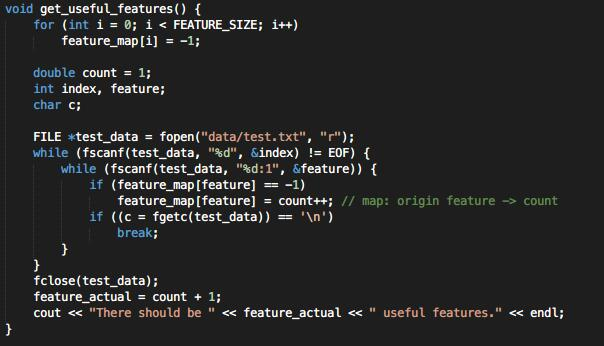
\includegraphics[width=384pt]{../results/code-preprocess.jpg}
	\caption{特征映射}
	\label{code:preprocess}
\end{figure}

经过实际运行,找到了\ 3183 个特性。之后在训练权值时,都需将现有特性转为新特性。

\subsection{并行化}

如果使用逻辑分类算法,由于计算所求的一组权值 $\theta{0}, \theta{1}, ..., \theta{N}$ 与整个训练数据集相关,无法并行计算。但如果同步计算两百多万条记录,耗时将会很长。为实现并行化,我将训练数据分成\ 4 万条记录一组的块,共\ 55 组;分别应用逻辑回归分类,可训练出\ 55 组参数。分别使用这\ 55 组参数预测测试数据集,可得到\ 55 组预测结果。综合这\ 55 组预测结果,加起来。再对每一条进行考虑,如果合值超过\ 27,那么该条测试记录的预测类别为 1,否则为 0。考虑到每个训练块的样本数量足够大,其训练出的参数与参考值应该是可靠的。

至于具体的实现,有多种方案可供选择:多线程、MPI、MapReduce(Hadoop)、Spark 等。由于个人计算机资源的限制,我选择使用多线程来实现并行化计算。OpenMP 是用于共享内存并行系统的多处理程序设计的一套指导性的编译处理方案,在现代很多编译器中都得到了实现。为并行计算这\ 55 组,只需在需要并行计算的块前添加\ \textbf{\#pragma omp parallel for}~\ref{code:openmp} 即可。

\begin{figure}[H]
	\centering
	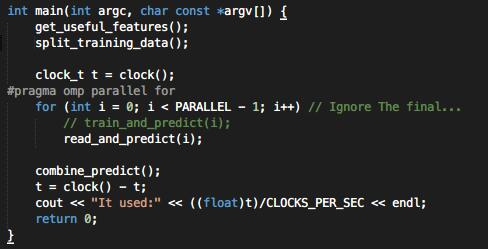
\includegraphics[width=384pt]{../results/code-openmp.jpg}
	\caption{OpenMP \#pragma}
	\label{code:openmp}
\end{figure}

\begin{description}
	\item [注意] 使用并行计算能加快计算速度,但得注意动态分配内存的问题,需要及时 delete。
\end{description}

我的 PC 处理器为 Intel(R) Core(TM) i5-3230M CPU @ 2.6GHz,双核,含 4 个超线程。在这台\ PC 上使用多线程完成参数训练与结果预测耗时,约为\ 8800 秒,近\ 3 个小时,CPU 占用为100\%,如图 ~\ref{fig:parallel} 。而不使用多线程时,CPU 占用为\%,如图~\ref{fig:noparallel}。考虑到时间问题,并没有测试具体耗时。

\begin{figure}[H]
	\centering
	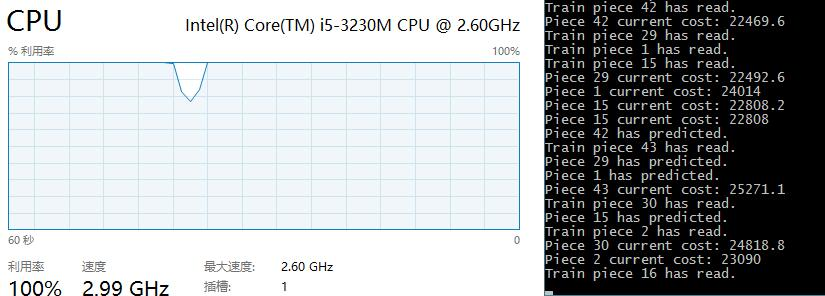
\includegraphics[width=384pt]{../results/parallel.jpg}
	\caption{并行}
	\label{fig:parallel}
\end{figure}

\begin{figure}[H]
	\centering
	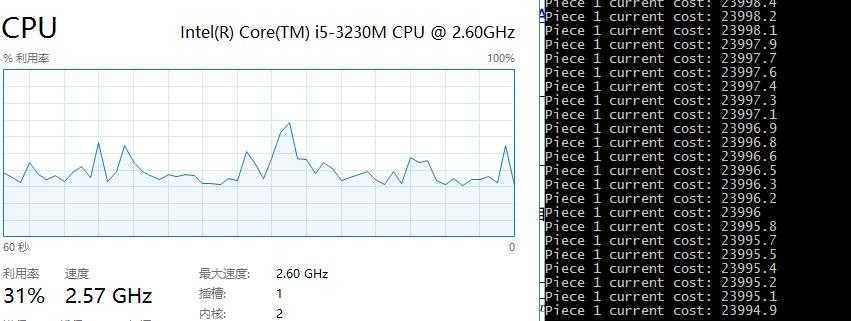
\includegraphics[width=384pt]{../results/noparallel.jpg}
	\caption{非并行}
	\label{fig:noparallel}
\end{figure}

\section{实验结果}

对本项目,我设置的\ $\alpha$ 值为 0.01,对应的预测结果在 Kaggle 上得到了\ $57.128\%$  的准确率,见图~\ref{fig:kaggle}。我的代码可在\  \href{https://github.com/daix6/Data-Mining/tree/master/hw2}{github} 看到。

\begin{figure}[H]
	\centering
	
\includegraphics[width=384pt]{../results/kaggle.jpg}
	\caption{Kaggle 准确率}
	\label{fig:kaggle}
\end{figure}

\section{总结}

\end{document}

